
Los Software, que estaremos utilizando son multiplataforma y se pueden instalar en Mac, Windows y Linux.

Las actividades que estaremos realizando durante en este capítulo son:
\textbf{
\begin{enumerate}
    \item Instalar el Software Visual Studio Code
    \item Instalar el Software Node.js
    \item Realizar un ejemplo básico con Node.js
    \item Instalar el Framework Electron y ejecutar un programa sencillo desde Visual Studio Code
    \item Empaquetar nuestra aplicación y convertirla en un ejecutable .exe
\end{enumerate}
}

\section{INSTALACIÓN DE VISUAL ESTUDIO CODE}
\begin{enumerate}
\item \hypertarget{instalarcode}{Para instalar \textbf{Visual Studio code}}, nos dirigiremos a la página oficial 
 \begin{minipage}[c]{0,17 \textwidth}
 \href{https://code.visualstudio.com/}{
 \def\svgwidth{0.9\textwidth}
 \input{IMGSVG/CLICAQUI.pdf_tex}} 
 \end{minipage}\newline \hyperlink{code}{\textcolor{red}{$\looparrowright$URL4$\looparrowleft$}}.
 Descargaremos la versión correspondiente a nuestro sistema operativo, simplemente damos clic y se descargará de inmediato.
\begin{figure}[H]
    \centering
    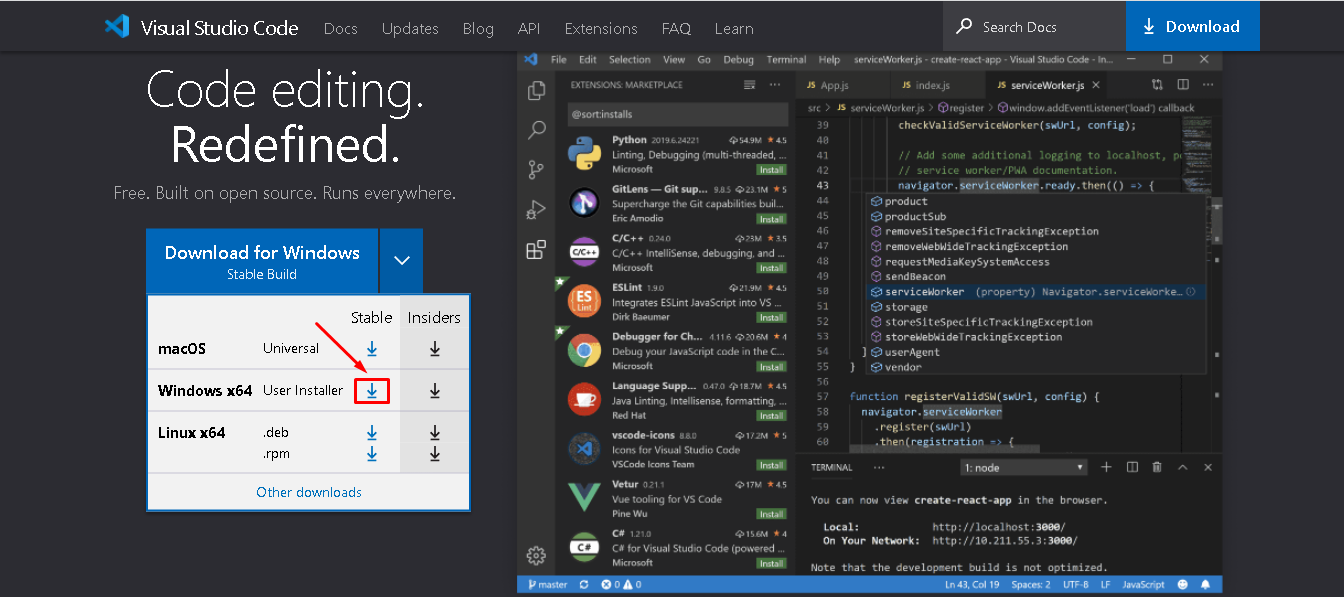
\includegraphics[width = 16 cm]{img/parte1code.png}
    \caption{DESCARGA DE VISUAL CODE}
\end{figure}
\newpage
\item Abrimos el ejecutable y aceptamos \textbf{los términos de licencia} y pulsamos \textbf{siguiente. }
\begin{figure}[H]
    \centering
    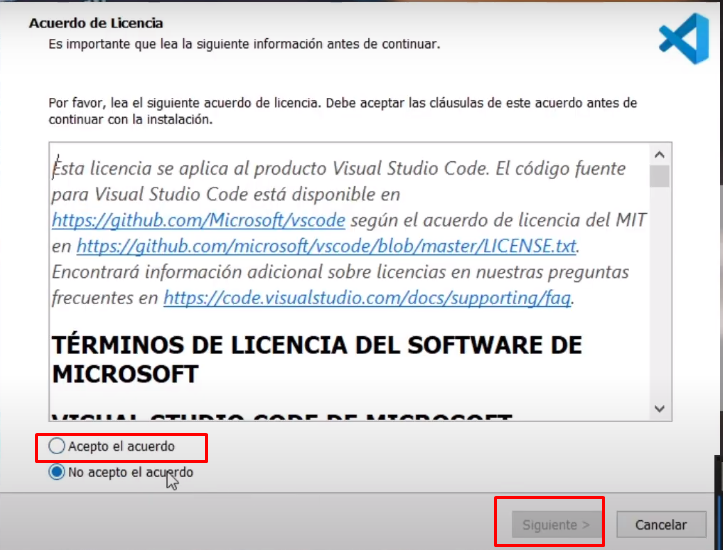
\includegraphics[width = 10 cm]{img/parte2code.png}
    \caption{TÉRMINOS DE LICENCIA}
\end{figure}
\item Elegimos el destino de instalación y pulsamos \textbf{siguiente. }
\begin{figure}[H]
    \centering
    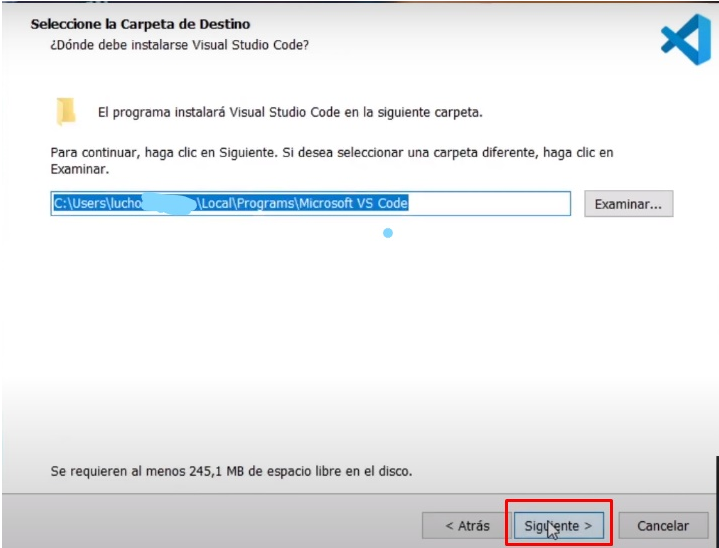
\includegraphics[width = 10 cm]{img/parte3codes.png}
    \caption{UBICACIÓN INSTALACIÓN}
\end{figure}
\newpage
\item Pulsamos \textbf{siguiente} a todo lo que venga y por último esperemos que termine de instalar 
\begin{figure}[H]
\centering
\begin{subfigure}{0.5\textwidth}
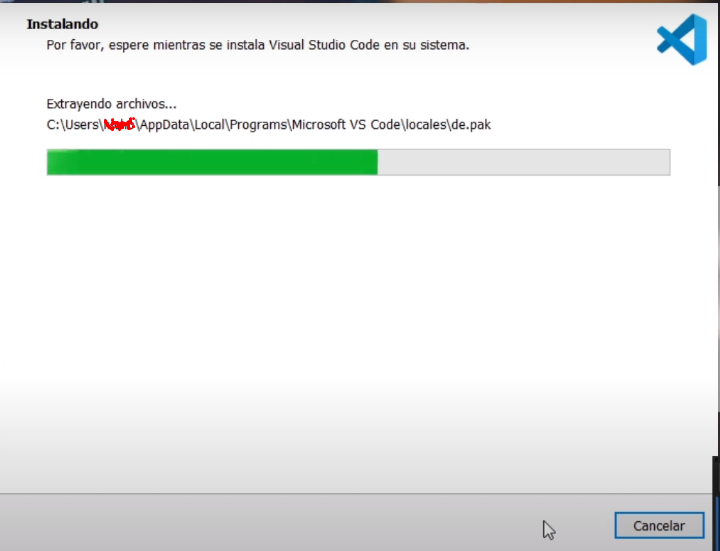
\includegraphics[width=6cm ]{img/CARGUECODE.png}
\end{subfigure}
\begin{subfigure}{0.5\textwidth}
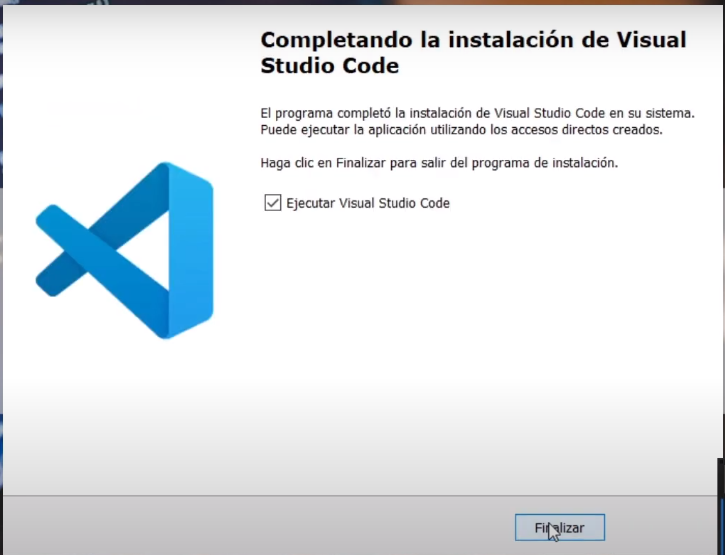
\includegraphics[width=6cm]{img/finalcode.png}
\end{subfigure}
\end{figure}

\item Una vez instalado \textbf{Visual Studio}, lo abrimos e instalaremos una extensión que nos servirá para colocarlo en español.Damos clic en \textbf{extensiones}.
\begin{figure}[H]
    \centering
    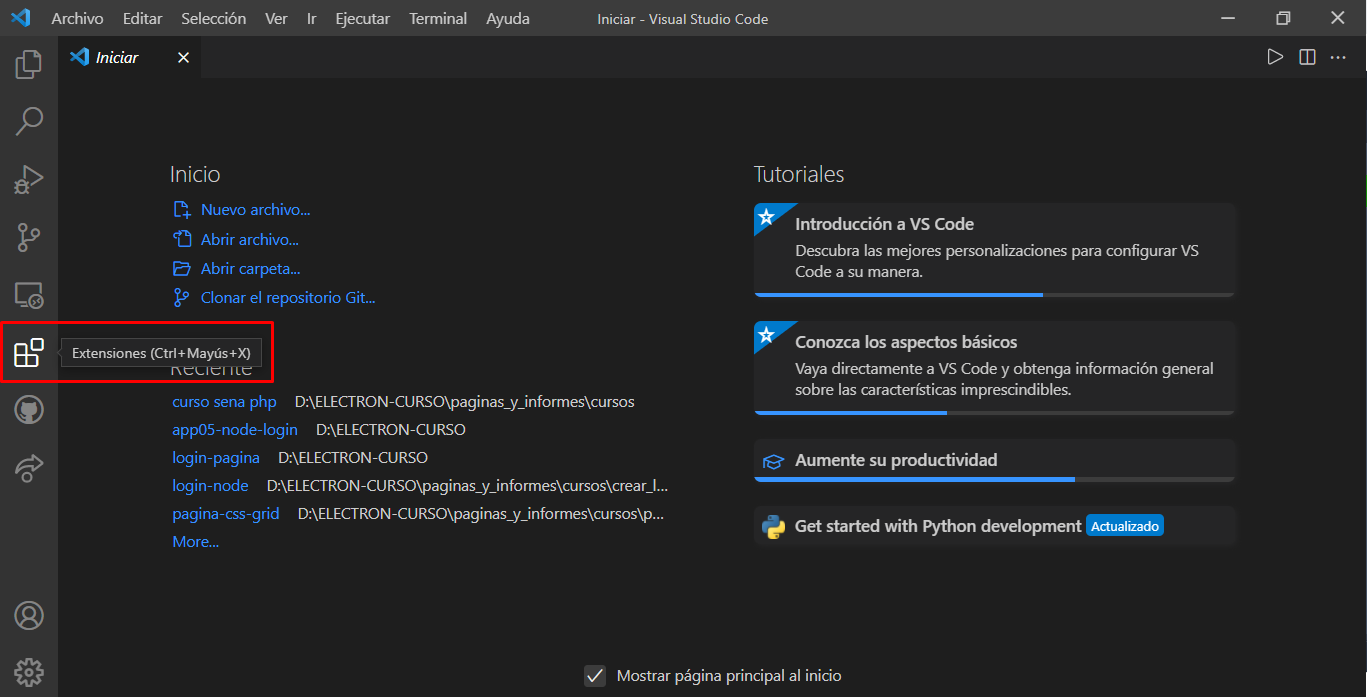
\includegraphics[width = 16 cm]{img/extensioncode.png}
    \caption{EXTENSIONES}
\end{figure}
\newpage
\item En la barra de búsqueda escribiremos \textbf{Spanish Language} damos clic en la primera opción y después \textbf{pulsamos instalar} y con esto ya tendremos instalado Visual Studio Code y configurado en Español.
\begin{figure}[H]
    \centering
    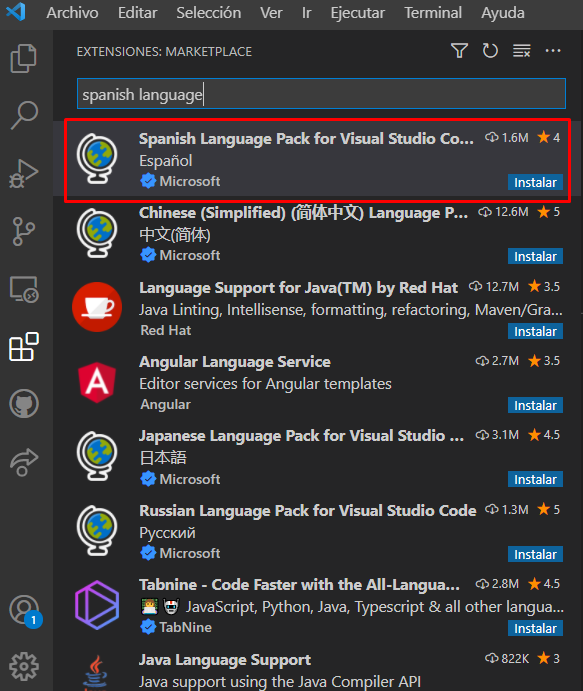
\includegraphics[width = 10 cm, height = 9cm]{img/final extension.png}
\end{figure}

\begin{figure}[H]
    \centering
    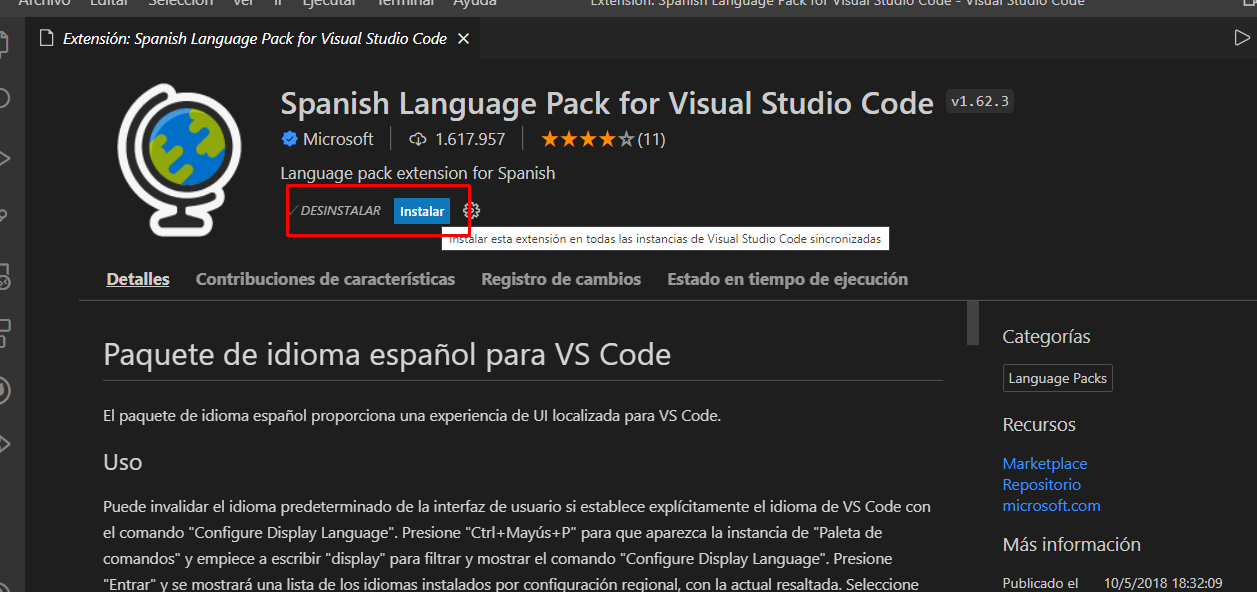
\includegraphics[width = 16 cm]{img/instalarexten.png}
\end{figure}
\end{enumerate}
\newpage
Algunas de las extensiones más importantes para \textbf{Visual Studio Code}, tenemos a:
\begin{itemize}
    \item  \textbf{vscode-icons}: nos ayudará a distinguir carpetas y tipos de archivos
    \item  \textbf{live server}: esta extensión nos permitirá lanzar un servidor local de desarrollo
    \item  \textbf{html snippets}: nos sirve para autocompletar código HTML
    \item  \textbf{prettier - Code formatter}:es un formateador de código obstinado. Aplica un estilo coherente al analizar su código y volver a imprimirlo con sus propias reglas que tienen en cuenta la longitud máxima de línea, ajustando el código cuando es necesario.
\end{itemize}

\section{INSTALACIÓN DE NODE.JS}
\begin{enumerate}
    \item \hypertarget{instalarnode}{Para instalar \textbf{Node.js}} nos vamos primero a la página oficial de Node.js,\begin{minipage}[c]{0,17 \textwidth}
 \href{https://nodejs.org/es/}{
 \def\svgwidth{0.9\textwidth}
 \input{IMGSVG/CLICAQUI.pdf_tex}} 
 \end{minipage}\newline \hyperlink{node1}{\textcolor{red}{$\looparrowright$URL5$\looparrowleft$}}. Estando dentro de la página descargaremos la versión correspondiente a nuestro sistema operativo. Hasta la fecha:\textbf{ 16/11/2021}, la última versión es:\textbf{ 17.1.0}, pero es recomendable descarga la versión: \textbf{ 16.13.0}.Por lo tanto, esta será versión que descargaremos.
    \begin{figure}[H]
    \centering
    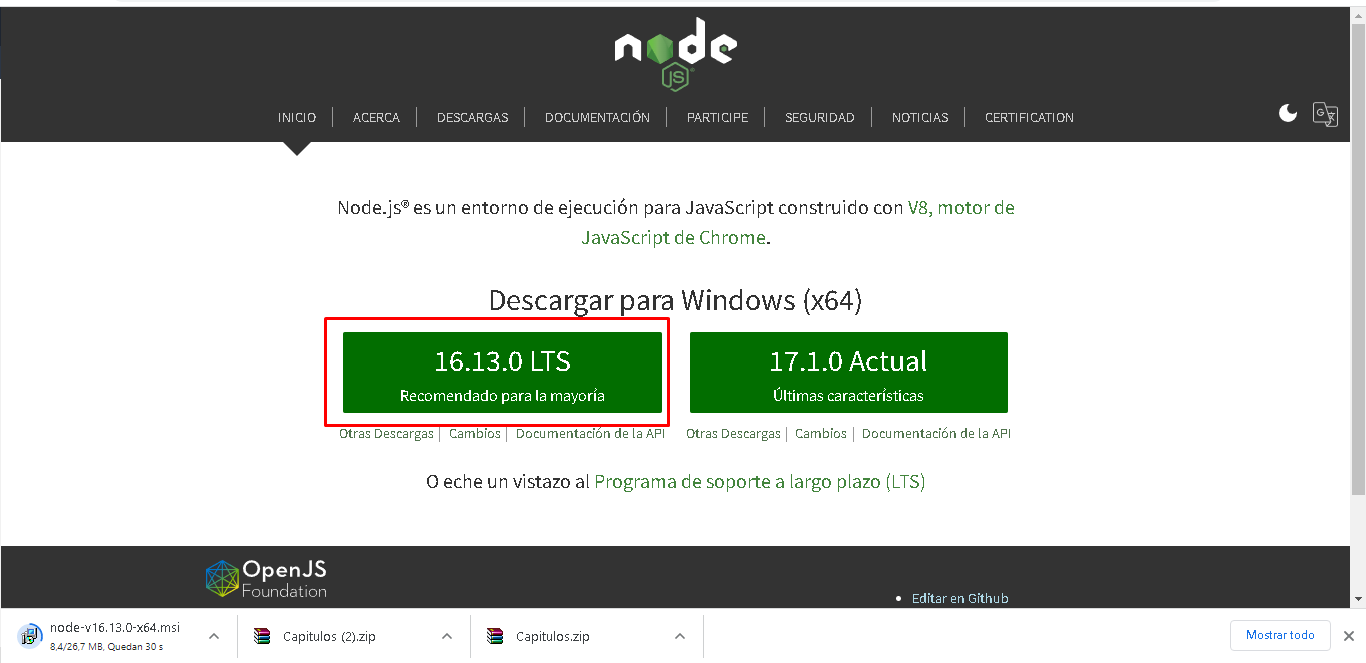
\includegraphics[width = 14 cm]{img/nodepagina.png}
    \caption{PÁGINA OFICIAL}
    \end{figure}
    \newpage
    \item Abrimos el ejecutable, damos clic en \textbf{Next}, 
    aceptamos los \textbf{términos de licencia} \newline y pulsamos de nuevo \textbf{Next}
\begin{center}
\begin{tabular}{p{6cm} p{6cm}}
\begin{minipage}[c]{6cm}
\centering
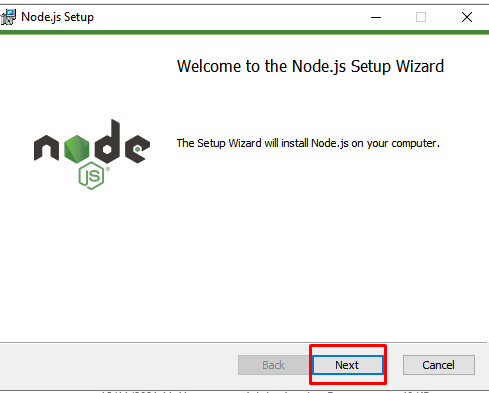
\includegraphics[width=1\textwidth]{img/node2.png}
\end{minipage}
&  \begin{minipage}[c]{6cm}
\centering
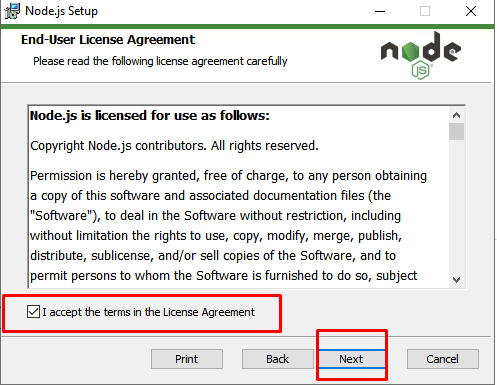
\includegraphics[width=1\textwidth]{img/node3.png}
\end{minipage}
\end{tabular}
\end{center}
  
    
   % \begin{center}
   % \begin{tabularx}{0.9\textwidth}{>{\raggedright\arraybackslash}X%>{\centering\arraybackslash}X}
    %\begin{minipage}{9cm}
    % 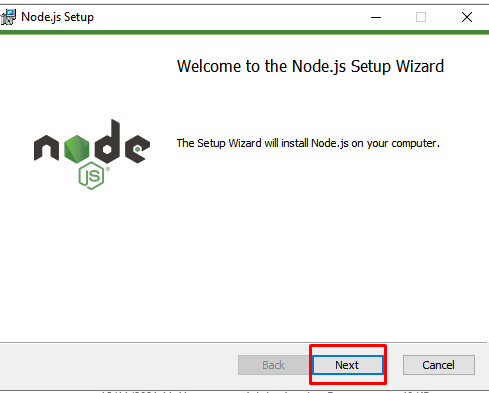
\includegraphics[width=0.6\textwidth]{img/node2.png%}
    % \end{minipage} & \begin{minipage}{9cm}
    % 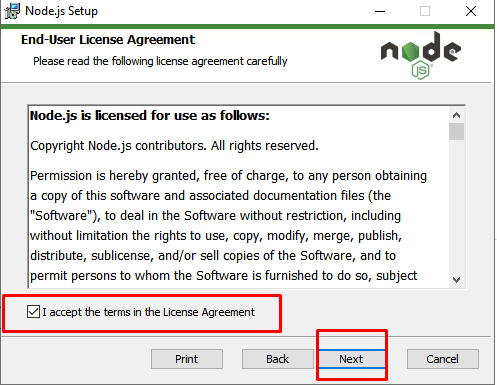
\includegraphics[width=0.6\textwidth]{img/node3.png%}
    % \end{minipage}
   % \end{tabularx}
    %\end{center}
    \item Ahora elegimos la ruta de instalación y pulsamos next
    \begin{figure}[H]
        \centering
        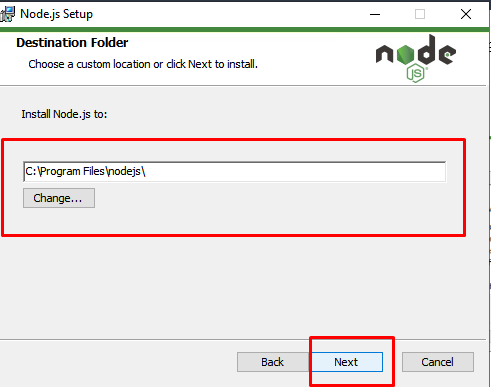
\includegraphics[width=0.7\textwidth]{img/node4.png}
    \end{figure}
    \newpage
    \item Elegimos los paquetes a instalar en este caso yo lo dejaré por defecto
    \begin{figure}[H]
        \centering
        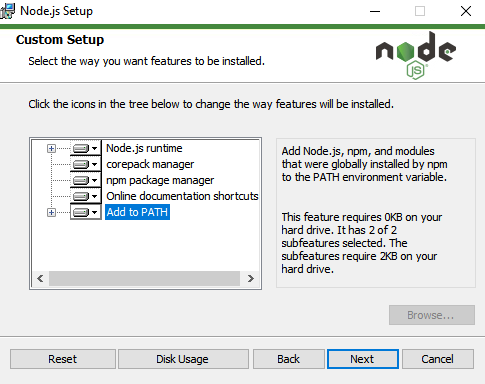
\includegraphics[width=0.7\textwidth]{img/NODE5.png}
    \end{figure}
    
    \item Nos ofrecerá instalar herramientas para compilar módulos nativos, por lo tanto, lo chuleamos y pulsamos \textbf{next }
    \begin{figure}[H]
        \centering
        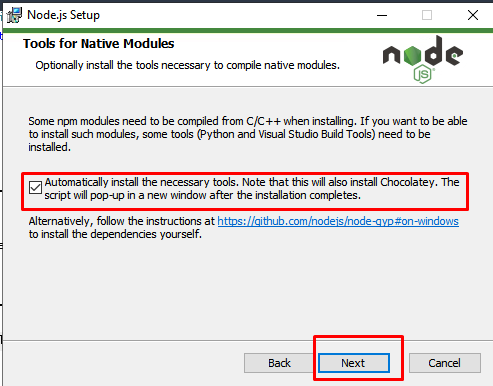
\includegraphics[width=0.7\textwidth]{img/node6.png}
    \end{figure}
    \newpage
    \item Por último le daremos \textbf{Install} y esperemos que instale 
    \begin{figure}[H]
        \centering
        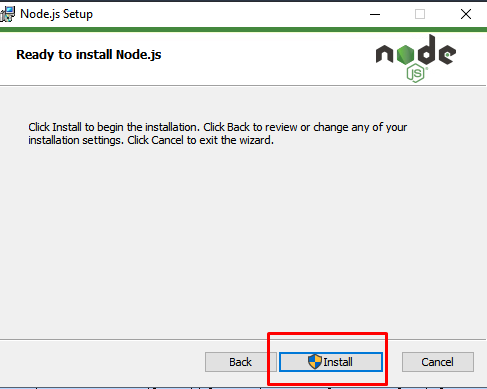
\includegraphics[width=0.7\textwidth]{img/node7.png}
    \end{figure}
    
    \begin{figure}[H]
        \centering
        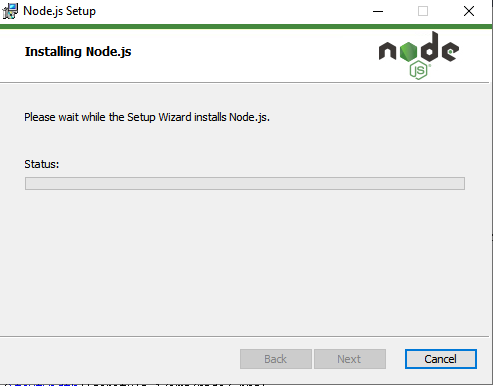
\includegraphics[width=0.7\textwidth]{img/node8.png}
    \end{figure}
    \newpage
      \item Después que termine de instalar le damos \textbf{Finish}
    \begin{figure}[H]
        \centering
        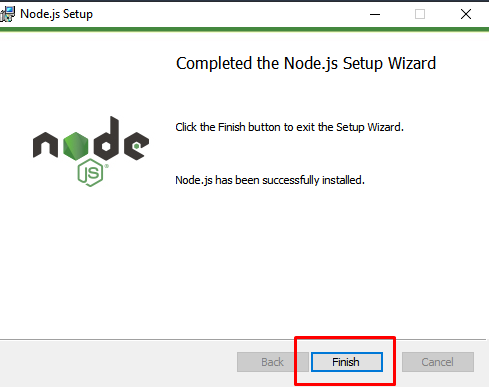
\includegraphics[width=0.7\textwidth]{img/node9.png}
    \end{figure}
    
      \item Para comprobar la instalación nos vamos a nuestra consola y escribiremos el siguiente comando: \textbf{node -v }.Nos debería aparecer la versión que tenemos instalada de Node.js \textbf{(en mi caso la versión 16.13.0)}. Para comprobar que se nos ha instalado también los paquetes NPM, escribiremos\textbf{ npm -v} y pulsaremos de \textbf{nuevo Enter}.Con esto ya hemos terminado la instalación de Node.js
    \begin{figure}[H]
        \centering
        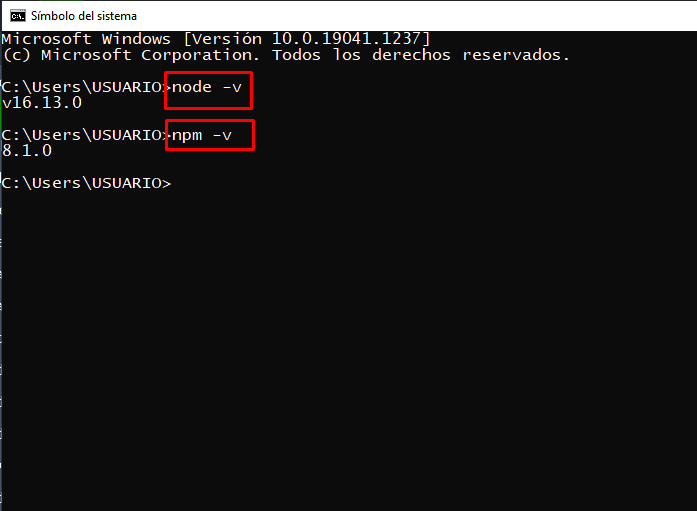
\includegraphics[width=0.6\textwidth]{img/node10.png}
    \end{figure}
    
\end{enumerate}
\newpage
\section{CREACIÓN DE UN PROGRAMA SENCILLO
UTILIZANDO NODE.JS }
\hypertarget{EJEMPLONODE}{
Para poder realizar este ejercicio necesitarás primero tener instalado los Software \textbf{ Node.js \hyperlink{instalarnode}{\textcolor{red}{ver instalación} \textcolor{red}{$\looparrowleft$}}} y el  editor de código \textbf{Visual Studio Code \hyperlink{instalarcode}{\textcolor{red}{ver instalación} \textcolor{red}{$\looparrowleft$}}}}


\subsection{CONCEJOS A SEGUIR}
Si quieres entender un poco más acerca de lo que haremos en esta actividad, te recomiendo que mires el video que se adjuntará a continuación.
\subsubsection{VIDEO EDUCATIVO}
 Se adjunta código QR y link de acceso al video

Para escanear la imagen, te recomiendo la siguiente app: Lector de código QR.

Se adjunta link:
 \begin{minipage}[c]{0,19 \textwidth}
 \href{https://play.google.com/store/apps/details?id=com.teacapps.barcodescanner}{
 
\includegraphics[width=0.9\textwidth]{img/google play.png}
 }\end{minipage}
 \hyperlink{linkapp}{\textcolor{red}{$\looparrowright$URL1$\looparrowleft$}}
\begin{center}
 \begin{figure}[H]
 \centering

\includegraphics[width=0.35\textwidth]{img/QR1.jpeg}
 \caption{EJEMPLO NODE.JS}
 \label{fig:NODEQR}
\end{figure}
\end{center}

Link de acceso al video

\begin{enumerate}
\renewcommand{\theenumi}{\Alph{enumi}} %Letras mayúsculas
    \item Node.js\begin{minipage}[c]{0,17 \textwidth}\href{https://youtu.be/wd8zf3D0jic}{
 \def\svgwidth{0.9\textwidth}
 \input{IMGSVG/VERVIDEO.pdf_tex}} 
 \end{minipage}\hyperlink{NODE2}{\textcolor{red}{$\looparrowright$URL3$\looparrowleft$}}
\end{enumerate}
\newpage
aquí va la explicación

\newpage
\section{INSTALACIÓN DE ELECTRON Y EJECUCIÓN DE
UN PROGRAMA DE ESCRITORIO SENCILLO, USANDO VISUAL STUDIO CODE y NODE.JS}

Para poder \textbf{Instalar Electron} y comenzar a desarrollar  aplicaciones de escritorio utilizando este \textbf{FrameworK}, necesitarás tener instalado los Software\textbf{ Node.js} y el  editor de código \textbf{Visual Studio Code}.
\subsection{CONCEJOS A SEGUIR}
Si quieres entender un poco más acerca de lo que haremos en esta actividad y de paso aprender más sobre Electron, te recomiendo que el siguiente curso que se adjuntará a continuación.
\subsubsection{CURSO EDUCATIVO}
 Se adjunta código QR y link de acceso al curso de electron

Para escanear la imagen, te recomiendo la siguiente app: Lector de código QR.

Se adjunta link:
 \begin{minipage}[c]{0,19 \textwidth}
 \href{https://play.google.com/store/apps/details?id=com.teacapps.barcodescanner}{
 
\includegraphics[width=0.9\textwidth]{img/google play.png}
 }\end{minipage}
 \hyperlink{linkapp}{\textcolor{red}{$\looparrowright$URL1$\looparrowleft$}}
\begin{center}
 \begin{figure}[H]
    \centering
 
\includegraphics[width=0.3\textwidth]{img/QR2.jpeg}   
    \caption{CURSO ELECTRON.JS}
 \label{fig:ELECTRONQR}
 \end{figure}
                                           
\end{center}

Link de acceso al curso de electron

\begin{enumerate}
\renewcommand{\theenumi}{\Alph{enumi}} %Letras mayúsculas
    \item  Electron.js\begin{minipage}[c]{0,17 \textwidth}\href{https://youtube.com/playlist?list=PL2PZw96yQChzi-lLw6rqqAPRkNXSOeqtr}{
 \def\svgwidth{0.9\textwidth}
 \input{IMGSVG/VERVIDEO.pdf_tex}} 
 \end{minipage}\hyperlink{CURSOELECTRON}{\textcolor{red}{$\looparrowright$URL2$\looparrowleft$}}
\end{enumerate}
\newpage
 Si deseas saber más sobre el \textbf{Framework Electron}, te dejaré el link de la página oficial,\newline \begin{minipage}[c]{0,17 \textwidth}
 \href{https://www.electronjs.org/}{
 \def\svgwidth{0.9\textwidth}
 \input{IMGSVG/CLICAQUI.pdf_tex}} 
 \end{minipage}\hyperlink{oficialpagina}{\textcolor{red}{$\looparrowright$URL6$\looparrowleft$}}. Aquí encontrarás toda la información y documentación necesaria para trabajar con este Framework
 
 \subsection{INICIO DE LA ACTIVIDAD PRINCIPAL}
 
Para realizar esta actividad nos guiaremos de un tutorial que nos brinda la propia página oficial de Electron:
  \begin{minipage}[c]{0,17 \textwidth}
 \href{https://www.electronjs.org/docs/latest/tutorial/quick-start}{
 \def\svgwidth{0.9\textwidth}
 \input{IMGSVG/CLICAQUI.pdf_tex}} 
 \end{minipage}\hyperlink{tutorial}{\textcolor{red}{$\looparrowright$URL7$\looparrowleft$}}.
\begin{enumerate}
    \item Crearemos una carpeta en nuestro escritorio, se le puede colocar el nombre que queramos.Ahora nos dirigimos a nuestro editor de código Visual Studio Code y abriremos esa carpeta
     \begin{figure}[H]
        \centering
        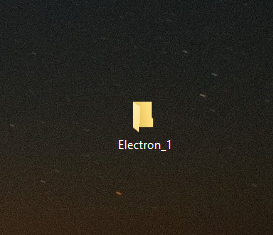
\includegraphics[width=0.3\textwidth]{img/electron0.png}
        \caption{CARPETA CREADA}
    \end{figure}
     \begin{figure}[H]
        \centering
        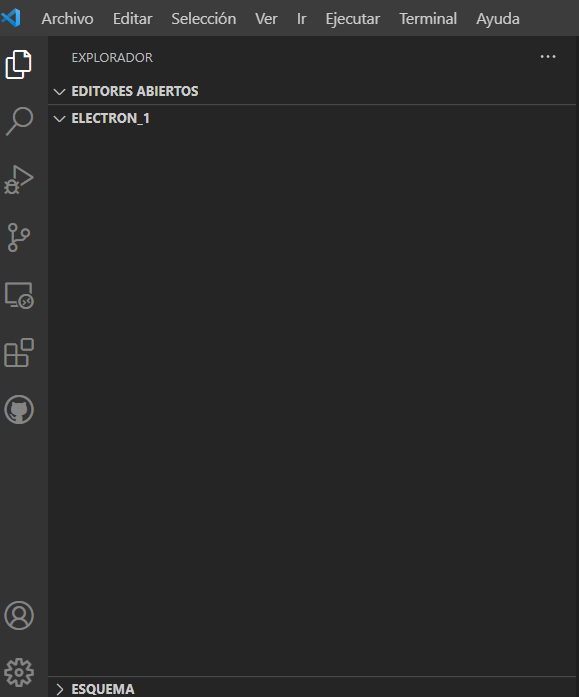
\includegraphics[width=0.4\textwidth]{img/electron1.png}
        \caption{ABRIENDO CARPETA DESDE VISUAL CODE}
    \end{figure}
     \subsubsection*{ESTRUCTURA BASE}
     
    \item Dentro de esta carpeta vamos a estar creando toda la estructura base que se encargara de la ejecución de nuestra aplicación electron.

    Dentro de nuestra carpeta estaremos creando los siguientes archivos:
    
    \begin{enumerate}
        \item \hypertarget{package}{\textbf{package.json}}: este es generado automáticamente cuando se instalan paquetes o dependencias \textbf{npm} en el proyecto. Su finalidad principal es mantener todo el historial de los paquetes instalados y optimizar la forma en que se generan las dependencias del proyecto.
        \item \hypertarget{main}{\textbf{main.js}}: este archivo será el punto de entrada del proyecto el que se encargara de arrancar el proceso principal de electron.
        \item \hypertarget{index}{\textbf{index.html}}: nos mostrará la vista de inicio de la aplicación. Podemos también crear archivos adicionales como \textbf{CSS, JavaScript}. permitiéndonos darle estructura, estilos e interactividad a nuestra principal.
    \end{enumerate}
    
    Al final nuestro directorio lucirá de la siguiente manera:
    
    your-app/
    
    $\vdash ${package.json}
    
    $\vdash ${main.js}
    
    $\llcorner${index.html}
    \newpage
    
    \subsubsection*{CREACIÓN DE LOS ARCHIVOS}
    
    \item Para crear el archivo \textbf{package.json} primero nos dirigimos a la opción \textbf{ver}, luego a \textbf{terminal}, esto nos integrará una terminal en nuestro proyecto, ubicándose en la ruta actual.
    \begin{figure}[H]
        \centering
        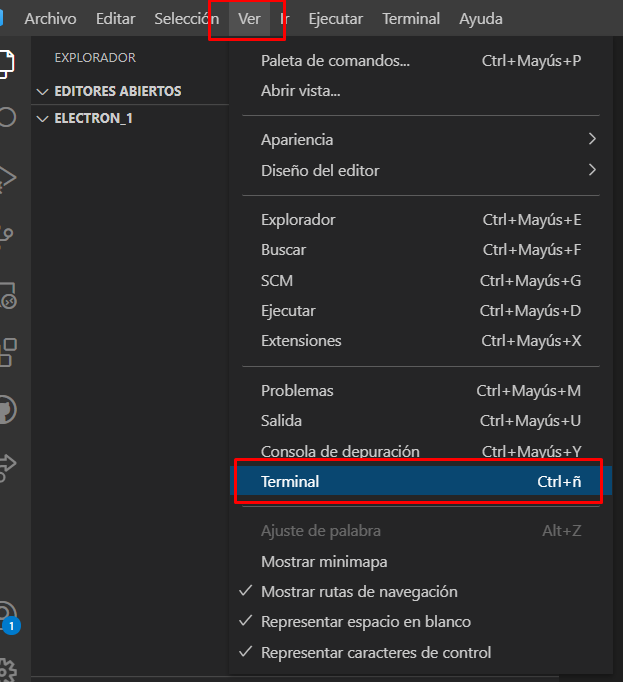
\includegraphics[width=0.6\textwidth]{img/electron2.png}
    \end{figure}
    \begin{figure}[H]
        \centering
        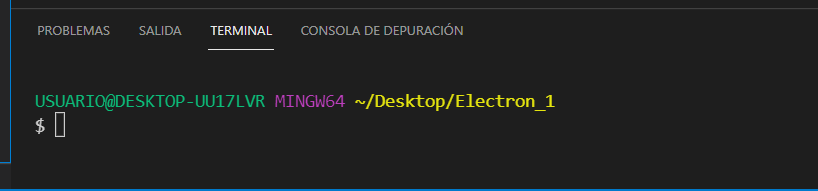
\includegraphics[width=0.8\textwidth]{img/electron3.png}
    \end{figure}
    \newpage
    \item Dentro de esta terminal escribiremos el siguiente comando:\textbf{ npm init --yes} y pulsamos \textbf{Enter}. Esto nos creará el archivo \textbf{package.json}
    \begin{figure}[H]
        \centering
        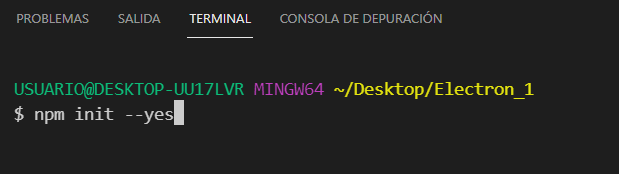
\includegraphics[width=0.8\textwidth]{img/electron4.png}
    \end{figure}
    \begin{figure}[H]
        \centering
        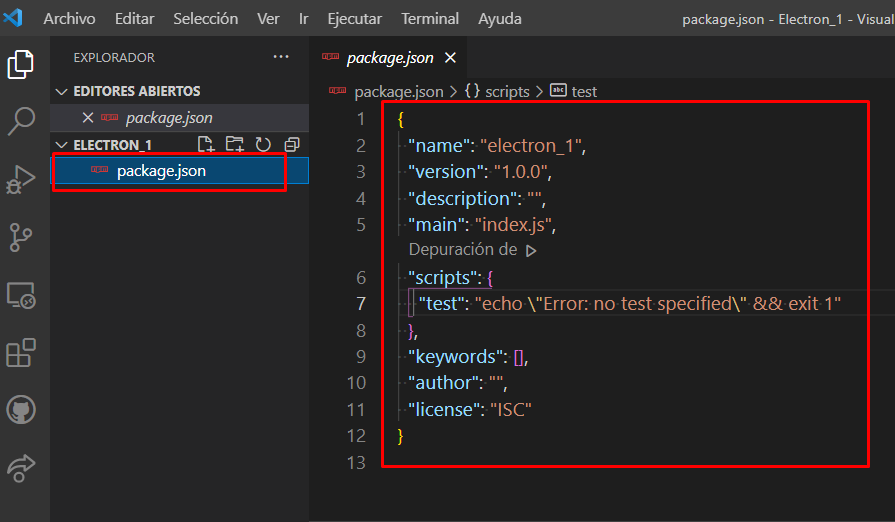
\includegraphics[width=0.9\textwidth]{img/electron5.png}
        \caption{ARCHIVO PACKAGE.JSON}
    \end{figure}
     \textbf{Campos más habituales de package.json:}
  \begin{itemize}
   \renewcommand{\labelitemi} {\textcolor{red}{$\bigstar$}}
      \item \textbf{name}: nombre del proyecto, librería o paquete.
      \item \textbf{version}: versión del paquete.
      \item \textbf{description}: descripción breve del paquete o proyecto.
      \item \textbf{main}: punto de entrada del proyecto. Suele ser index.js (node) o index.html (browser).
      \item \textbf{scripts}: colección de scripts del proyecto. Aquí colocaremos los comandos que nos ayudaran a correr nuestro programa durante la fase de desarrollo. 
      \item \textbf{keywords}: palabras clave relacionadas con el proyecto.
      \item \textbf{author}: nombre del autor del paquete.
      \item \textbf{license}: tipo de licencia del paquete o proyecto.
      % FUENTE https://lenguajejs.com/npm/administracion/package-json/ ENTRA AQUI ANDRES
      las veremos más adelante cuando se comiencen a instalar \textbf{paquetes npm}
      
      \item \textbf{dependencies}: colección de paquetes para producción y la versión instalada.Estas son obligatorias en nuestro proyecto  ya que son parte de la lógica de tu aplicación y son necesarias para que el proyecto funcione correctamente en producción
      \item \hypertarget{thesentence}{\textbf{devDependencies}}: colección de paquetes para desarrollo y la versión instalada.No son necesarias en producción y tu aplicación puede funcionar si ellas.
  \end{itemize}
  
  \item Ahora para tener más organizado el proyecto crearemos un directorio de nombre \textbf{src}, dentro de este se encontrará toda la estructura de proyecto, por lo tanto, en \textbf{src} crearemos una carpeta de nombre \textbf{views} aquí colocaremos todos los archivos \textbf{JS, HTML, CSS, IMÁGENES} necesarios para darle estructura, estilos e interactividad a la aplicación de escritorio.
   \begin{figure}[H]
        \centering
        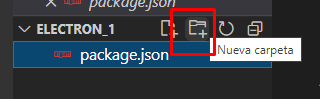
\includegraphics[width=0.4\textwidth]{img/electron6.png}
        \caption{CLIC EN CREAR CARPETA Y DESPUÉS ASIGNAMOS NOMBRE }
    \end{figure}
    \begin{figure}[H]
        \centering
        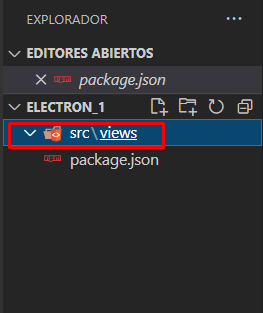
\includegraphics[width=0.4\textwidth]{img/electron7.png}
        \caption{CARPETAS CREADAS}
    \end{figure}
    \newpage
    \item Ahora lo que haremos será instalar\textbf{ Electron} como\hyperlink{thesentence}{\textcolor{red}{\textbf{ devDependencies}}}.Para eso primero nos dirigimos a la terminal de comando que tenemos integrada en nuestro proyecto y digitamos lo siguiente: \textbf{npm install --save-dev electron} y pulsamos \textbf{Enter} y esperamos que instale Electron.
    
      \begin{figure}[H]
        \centering
        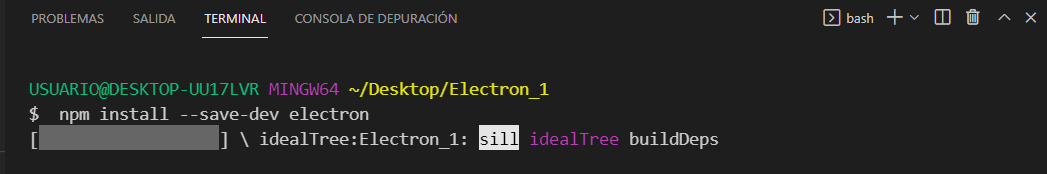
\includegraphics[width=0.9\textwidth]{img/electron8.png}
        \caption{INSTALACIÓN DE ELECTRON}
    \end{figure}
    
    \item Si la instalación se realizó correctamente en nuestro archivo\hyperlink{package}{\textcolor{red}{\textbf{ package.json}}} nos aparecerá la confirmación y además de eso en nuestro directorio automáticamente se creara una carpeta de nombre \textbf{node\_modules} aquí es donde se almacenan todas las dependencias y librerías que estaremos instalando mediante comandos \hyperlink{camannpm}{\textcolor{red}{\textbf{npm }}}y que más adelante estaremos utilizando en nuestro proyecto.Por ejemplo dentro de esta carpeta encontraremos el paquete de Electron que acabamos de instalar.  
  
\begin{figure}[H]
 \centering
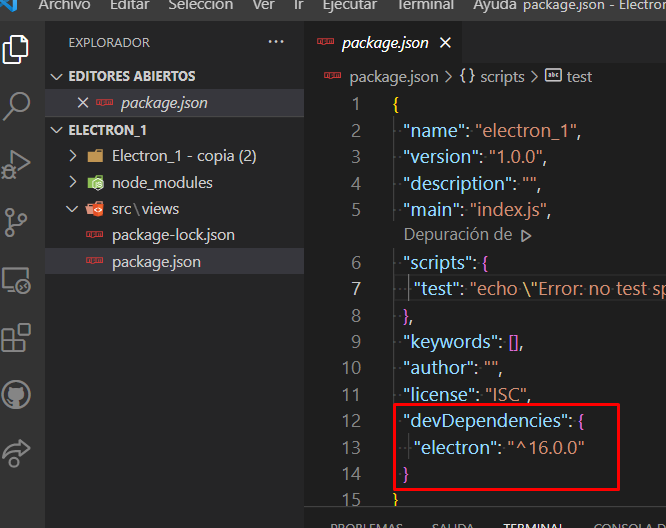
\includegraphics[width=0.7\textwidth]{img/electron9.png}
\caption{CONFIRMACIÓN INSTALACIÓN}
\end{figure}
\begin{figure}[H]
\centering
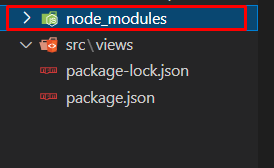
\includegraphics[width=0.8\textwidth]{img/electron10.png}   
\caption{CARPETA NODE\_ MODULE}
\end{figure}
\begin{figure}[H]
\centering
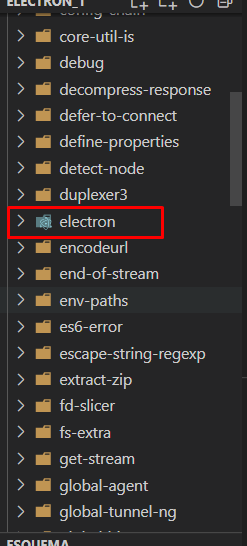
\includegraphics[width=0.3\textwidth]{img/electron11.png}   
\caption{PAQUETE DE ELECTRON}
\end{figure}
\newpage
\item Crearemos dos archivos vacíos.Uno de nombre: \hyperlink{main}{\textcolor{red}{\textbf{main.js}}}, dentro de \textbf{src} y otro de nombre: \hyperlink{index}{\textcolor{red}{\textbf{index.html}}} dentro de la carpeta \textbf{views}.
\begin{figure}[H]
 \centering
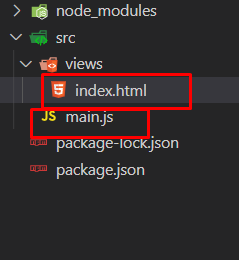
\includegraphics[width=0.3\textwidth]{img/electron12.png}

\end{figure}
\newpage

\item Ahora realizaremos algunas modificaciones 
 en el archivo\newline \textbf{ package.json}


%\lstset{language=, breaklines=true, basicstyle=\footnotesize}
%\lstset{numbers=left, numberstyle=\tiny, stepnumber=1, numbersep=-2pt}
\lstinputlisting[language=,]{packagejson.m}

\begin{enumerate}
    \item 
\end{enumerate}

\end{enumerate}


%https://www.lawebdelprogramador.com/foros/TeX-Latex/1464913-Incluir-Imagen-con-Texto.html

%https://www.overleaf.com/learn/latex/Tables

%https://manualdelatex.com/simbolos

%https://newbedev.com/how-to-use-figure-inside-a-minipage

%codigo de importancia para la creacion de imagenes
%\begin{center}
%begin{tabular}{c c }
        %\begin{minipage}{5 cm}
                         %\centering
                         %\begin{figure}[H]
                         %\centering
                         %
\includegraphics[width=0.9\textwidth]{img/QR1.jpeg}
                         %\caption{NODEJS}
                         %\label{fig:NODEQR}
                         %\end{figure}
                         %\end{minipage}  &   \begin{minipage}{5 cm}
                                             %\centering
                                             %\begin{figure}[H]
                                             %\centering
                                             %
\includegraphics[width=0.9\textwidth]{img/QR2.jpeg}   
                                             %\caption{ELECTRONJS}
                                             %\label{fig:ELECTRONQR}
                                             %\end{figure}
                                             %\end{minipage}\\
%\end{tabular}
%\end{center}